

\documentclass{beamer}

\mode<presentation> {

%\usetheme{Boadilla}  %MAYBE THIS
\usetheme{CambridgeUS} %MAYBE THIS


%\usecolortheme{dolphin}

\usecolortheme{seahorse}

}

\usepackage{graphicx} % Allows including images
\usepackage{booktabs} % Allows the use of \toprule, \midrule and \bottomrule in tables
\usepackage{hyperref}

\title[HTTP and REST]{HTTP and RESTful Implementation} % The short title appears at the bottom of every slide, the full title is only on the title page

\author{Sainyam Kapoor} % Your name



\institute[IIT-(BHU)] % Your institution as it will appear on the bottom of every slide, may be shorthand to save space
{
\includegraphics[width=15mm]{IITBHU_Logo_Matlab.png}\\
Indian Institute of Technology-(BHU),Varanasi \\ % Your institution for the title page
\medskip

\textit{sainyam.kapoor.cse12@iitbhu.ac.in} % Your email address
}
\date{March 2014} % Date, can be changed to a custom date

\begin{document}

\begin{frame}
\titlepage % Print the title page as the first slide
\end{frame}

\begin{frame}
\frametitle{Overview} % Table of contents slide, comment this block out to remove it
\tableofcontents % Throughout your presentation, if you choose to use \section{} and \subsection{} commands, these will automatically be printed on this slide as an overview of your presentation
\end{frame}

%----------------------------------------------------------------------------------------
%	PRESENTATION SLIDES
%----------------------------------------------------------------------------------------

%------------------------------------------------
\section{HTTP} % Sections can be created in order to organize your presentation into discrete blocks, all sections and subsections are automatically printed in the table of contents as an overview of the talk
%------------------------------------------------

\subsection{Introduction to Hypertext Transfer Protocol} % A subsection can be created just before a set of slides with a common theme to further break down your presentation into chunks

\begin{frame}
\frametitle{Introduction to Hypertext Transfer Protocol}
HTTP (Hypertext Transfer Protocol) is perhaps the most popular application protocol used in the Internet.\\


\begin{itemize}
\item HTTP is an asymmetric request-response client-server protocol as illustrated.  An HTTP client sends a request message to an HTTP server.  The server, in turn, returns a response message.  In other words, HTTP is a pull protocol, the client pulls information from the server . 
\begin{figure}[ht!]
\centering
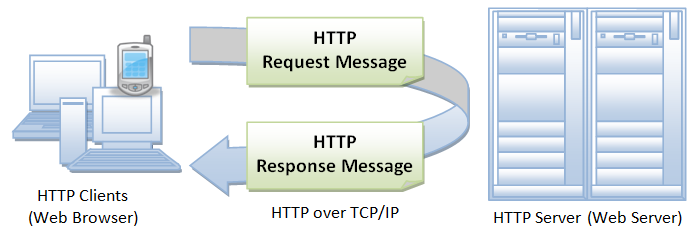
\includegraphics[width=90mm]{HTTP1.jpg}
\caption{Flow}
\label{overflow}
\end{figure}
\end{itemize}
\end{frame}

%------------------------------------------------

\begin{frame}
\frametitle{Introduction to HTTP(cont.)}
\begin{itemize}
\item HTTP is a stateless protocol. In other words, the current request does not know what has been done in the previous requests.
\item HTTP permits negotiating of data type and representation, so as to allow systems to be built independently of the data being transferred.
\end{itemize}
\end{frame}

%------------------------------------------------
\subsection{RFC2616-Hypertext Transfer Protocol}
%------------------------------------------------

\begin{frame}
\frametitle{RFC2616- Defined Standard For HTTP/1.1}
HTTP has been in use by the World-Wide Web global information initiative since 1990. This specification defines the protocol referred to as "HTTP/1.1",
\begin{itemize}
\item Quoting from the RFC2616: "The Hypertext Transfer Protocol (HTTP) is an application-level protocol for distributed, collaborative, hypermedia information systems. It is a generic, stateless, protocol which can be used for many tasks beyond its use for hypertext, such as name servers and distributed object management systems, through extension of its request methods, error codes and headers."

\end{itemize}
\end{frame}

%------------------------------------------------

\subsection{HTTP Request Structure}
%------------------------------------------------

\begin{frame}
\frametitle{HTTP Request Structure}
The beginning of the HTTP request will have the request line, which will be followed by up to three headers: a general header, a request header, and an entity header. \\~\\After that will be the message body. \\~\\The request line specifies the method type (such as GET or POST), the URI requested, and the version of HTTP to use (the current standard is 1.1).

\end{frame}

%------------------------------------------------
%------------------------------------------------

\begin{frame}
\frametitle{HTTP Response Structure(Example)}
Here's a simple HTTP Response
\begin{figure}[ht!]
\centering
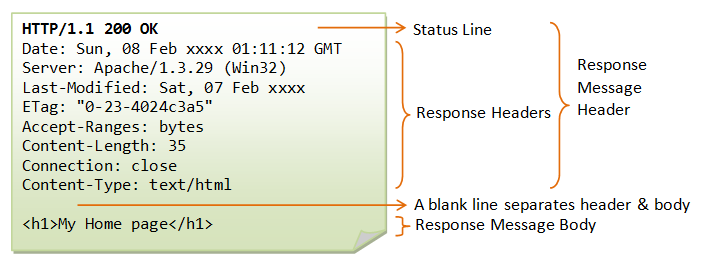
\includegraphics[width=90mm]{HTTP_Response.png}
\caption{A Simple Response}
\label{overflow}
\end{figure}
\end{frame}

%------------------------------------------------

\subsection{HTTP Request Methods}
%------------------------------------------------

\begin{frame}
\frametitle{HTTP Verbs all the way}
\begin{itemize}

\item GET: A client can use the GET request to get a web resource from the server.

\item POST: Used to post data up to the web server.
\item PUT: Ask the server to store the data.
\item DELETE: Ask the server to delete the data.
\end{itemize}
\end{frame}

%------------------------------------------------

\begin{frame}
\frametitle{HTTP Verbs(Others)}
\begin{itemize}


\item HEAD: A client can use the HEAD request to get the header that a GET request would have obtained. Since the header contains the last-modified date of the data, this can be used to check against the local cache copy.
\item TRACE: Ask the server to return a diagnostic trace of the actions it takes.
\item OPTIONS: Ask the server to return the list of request methods it supports.
\item CONNECT: Used to tell a proxy to make a connection to another host and simply reply the content, without attempting to parse or cache it. This is often used to make SSL connection through the proxy.
\end{itemize}
\end{frame}


%------------------------------------------------
\section{RESTFul Implementation }
%------------------------------------------------
\subsection{Introduction to RESTFul Implementation} 
\begin{frame}
\frametitle{RESTFul Implementation}
\begin{tabular}{@{\hspace{2ex}}p{30em}}
Representational State Transfer a.k.a. REST is a software architecture style that centers around the transmission of data over HTTP, using only the four basic HTTP verbs. It also deliberately avoids the use of any additional wrappers such as a SOAP envelope and the use of any state data.\\~\\
An Example:\\~\\The World Wide Web: Web browsers act as clients accessing resources hosted on Web servers. The resources are represented using HTML or XML grammars that all Web browsers can consume. The browsers can also easily follow the links to new resources.
\end{tabular}
\end{frame}

%------------------------------------------------
\subsection{Why REST? | What is REST?}
%------------------------------------------------

\begin{frame}
\frametitle{Why REST? | What is REST?}
\begin{itemize}
\item REST attempts to minimize latency while maximizing scalability.
\item REST is a Style
\item REST is a set of six constraints (one optional)
\item An API is NOT RESTful if it is not adhering to these constraints which is not necessarily a bad thing.
\item While REST provides a number of benefits, it may not be the right Architectural Style for a given project

\end{itemize}
\end{frame}

%------------------------------------------------
%------------------------------------------------
\subsection{What REST is not}
%------------------------------------------------

\begin{frame}
\frametitle{What REST is NOT:}
\begin{itemize}
\item URIs
\item Identifying Resources
\item Designing Responses (XML, JSON, XHTML, HAL)
\item HTTP Verbs (GET, PUT, POST, DELETE,….)
\item Headers (Caching)
\item HTTP Response Codes

\end{itemize}
\end{frame}

%------------------------------------------------
%------------------------------------------------

\begin{frame}
\frametitle{Some Characteristics of REST}
\textbf{Client-server Architecture}
\begin{tabular}{@{\hspace{3ex}}p{30em}}
\begin{itemize}
\item A server component offering services, listens for requests upon these services. A client component desires that a service be performed, sends a request to the server via a connector.
\end{itemize}
\begin{figure}[ht!]
\centering
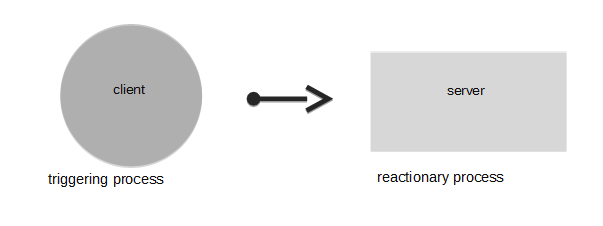
\includegraphics[width=100mm]{rest1.png}

\end{figure}
This separation allows for the two components to evolve independently, which increases scalability.
\end{tabular}
\end{frame}

%------------------------------------------------
%------------------------------------------------

\begin{frame}
\frametitle{Some Characteristics of REST(cont.)}
\textbf{Stateless Communication}
\\~\\
\begin{tabular}{@{\hspace{3ex}}p{30em}}
Each request from the client must contain all necessary information to understand the request.
\\
This constraint induces:
\begin{itemize}
\item Visibility – need to look at only one request to get the full nature of the request
\item Reliability – eases the task of recovering from failures
\item Scalability – not having to store data between requests allows the server to free resources


\end{itemize}
\end{tabular}

\end{frame}

%------------------------------------------------
%------------------------------------------------

\begin{frame}
\frametitle{Some Characteristics of REST(cont.)}
\textbf{Cache}
\\~\\
\begin{tabular}{@{\hspace{3ex}}p{28em}}
Cache constraints require that the data within a response to a request be labeled as cacheable or non-cacheable. If a response is cache-able, a client cache is given the right to reuse the response data for later, equivalent requests.
\\~\\
Cache constraints eliminate some interactions and improve efficiency and scalability.Cache can decrease reliability because of stale data.

\end{tabular}
\end{frame}

%------------------------------------------------

%------------------------------------------------

\begin{frame}
\frametitle{Some Characteristics of REST(cont.)}
\textbf{Uniform Interface}
\\~\\

\begin{itemize}
\item Identification of resources \\ \ Are sources is any information that can be named. An example of a\\ \  resource is the current weather in Varanasi,Uttar Pradesh.\\ \ Resource identification requires the same authority who maintains \\ \ the reference to a resource to also be responsible for preserving\\ \  meaning of that resource.
\item Manipulation of resources through representations \\ \ The resources must be manipulated via representations. A client has\\ \   no access to a resource directly, it can only send and receive \\ \  representations from the server. (An-example of a representation is an \\ \  HTML page with a PNG image of the current weather in Varanasi,UP.)
\item Self-descriptive messages\\ \ States that all messages must include meta-data which describe\\ \ the meaning of the message.

\end{itemize}


\end{frame}

%------------------------------------------------


%------------------------------------------------

\begin{frame}
\frametitle{Some Characteristics of REST(cont.)}
\textbf{Layered System}
\\~\\
\begin{tabular}{@{\hspace{3ex}}p{28em}}
Layered system style allows an architecture to be composed of hierarchical layers by constraining component behavior so each component cannot ‘see’ beyond the immediate layer with which they are interacting.
\\~\\
Layered system style helps reduce complexity and promote independence. Layers can be used to protect new services from legacy clients.They can also add overhead.
\end{tabular}

\end{frame}

%------------------------------------------------


%------------------------------------------------

\begin{frame}
\frametitle{Some Characteristics of REST(cont.)}
\textbf{Code on Demand(Optional)}
\\~\\
\begin{tabular}{@{\hspace{3ex}}p{28em}}
REST allows client functionality to be extended by downloading and executing code in the form of scripts
\end{tabular}

\end{frame}

%------------------------------------------------

\section{References And Papers Discussed}


\begin{frame}
\frametitle{Contents Of Papers Discussed}
\textbf{Architectural Styles and
the Design of Network-based Software Architectures}
\\
By - Roy Thomas Fielding(2000)
\\Can be accessed from \url{https://www.ics.uci.edu/~fielding/pubs/dissertation/top.htm}
\\
\begin{tabular}{@{\hspace{3ex}}p{28em}}
This Paper investigates methods for determining how best to partition a system, how components identify and communicate with each other, how information is communicated, how elements of a system can evolve independently, and how all of the above can be described using formal and informal notations. An architectural style is a named, coordinated set of architectural constraints.
\end{tabular}

\end{frame}




\begin{frame}
\frametitle{Contents Of Papers Discussed(2)}
\textbf{ Hypertext Transfer Protocol -- HTTP/1.1}
\\
By - R. Fielding, J. Gettys, J. Mogul, H. Frystyk and T. Berners-Lee 
\\~\\
\begin{tabular}{@{\hspace{3ex}}p{28em}}
This document specifies an Internet standards track protocol for the
   Internet community, and requests discussion and suggestions for
   improvements. 
\end{tabular}

\end{frame}
%------------------------------------------------

\begin{frame}
\frametitle{References}
Architectural Styles and the Design of Network-based Software Architectures\\
\ \url{http://www.ics.uci.edu/~fielding/pubs/dissertation/top.htm}

Implementing Rest\\
\ \url{https://code.google.com/p/implementing-rest/}

Classification of HTTP-based APIs\\
\ \url{http://www.asp.net/web-api/overview}
\\RFC-2616\\
\ \url{https://www.ietf.org/rfc/rfc2616.txt}
Representational State Transfer (REST) (Chapter -5)
\ \url{https://www.ics.uci.edu/~fielding/pubs/dissertation/top.htm}

\end{frame}
%------------------------------------------------

\begin{frame}
\Huge{\centerline{The End}}

\Huge{\centerline{Thank You!}}
\end{frame}

%----------------------------------------------------------------------------------------\%------------------------------------------------







\end{document} 